
%!TEX root = ../report.tex


% klar pointe: De væsentligste jobs i staten har tendens til at være lukkede om sig selv: det er i det private samt i de senere-statsliggjorte omsorgsjobs, der tidligere befandt sig i hjemmet, at der er cirkulation. 




%%%%%%%%%%%%%%%%%%%%%%%%%%%%%%%%%%%%%%%%%%%%%%
\chapter{Delanalyse 3:  \label{kapitel_delanalyse3_klasser}}
%%%%%%%%%%%%%%%%%%%%%%%%%%%%%%%%%%%%%%%%%%%%%%



\begin{tcolorbox}[title=Forskningspørgsmål 2,
subtitle style={boxrule=0.4pt} ]
  Kan forskelle i de sociale processer vise, at der er tale om segmenter, og ikke blot delmarkeder?
\end{tcolorbox}



%%%%%%%%%%%%%%%%%%%%%%%%%%%%%%%%%%%%%%%%%%%%%%
\section{bla blah}
%%%%%%%%%%%%%%%%%%%%%%%%%%%%%%%%%%%%%%%%%%%%%%
 
Ved hjælp af kortet kan vi se, at Oeschs definition af den manuelle arbejderklasses mobilitetsmønstre i høj grad stemmer overens med mobilitetsmønstre, der bekræftiger denne klasses barrierer i forhold til andre klasser: Dette gælder både i forhold til dens højere og lavere klassefraktion. Indenfor denne skelnen mellem to klassefraktioner, ser vi dog klassen delt op i segmenter, vis genstandsfelt i høj grad er afgrænset af færdigheder indenfor en specifik form for produktion. Det er denne, noget kompakte formulering, jeg nu vil uddybe for læseren. I figur \ref{fig delanalyse3 klasse manuelt ikkemanuel} er den manuelle arbejderklasse i Oesch skema fremhævet. 


%
   \begin{figure}[H]
   \begin{centering}
    \caption[Netværkskort: Manuel arbejderklasse - andre klasse]{Den manuelle arbejderklasse i Oesch klasseskema (rød) overfor de andre klasser (grå).}
    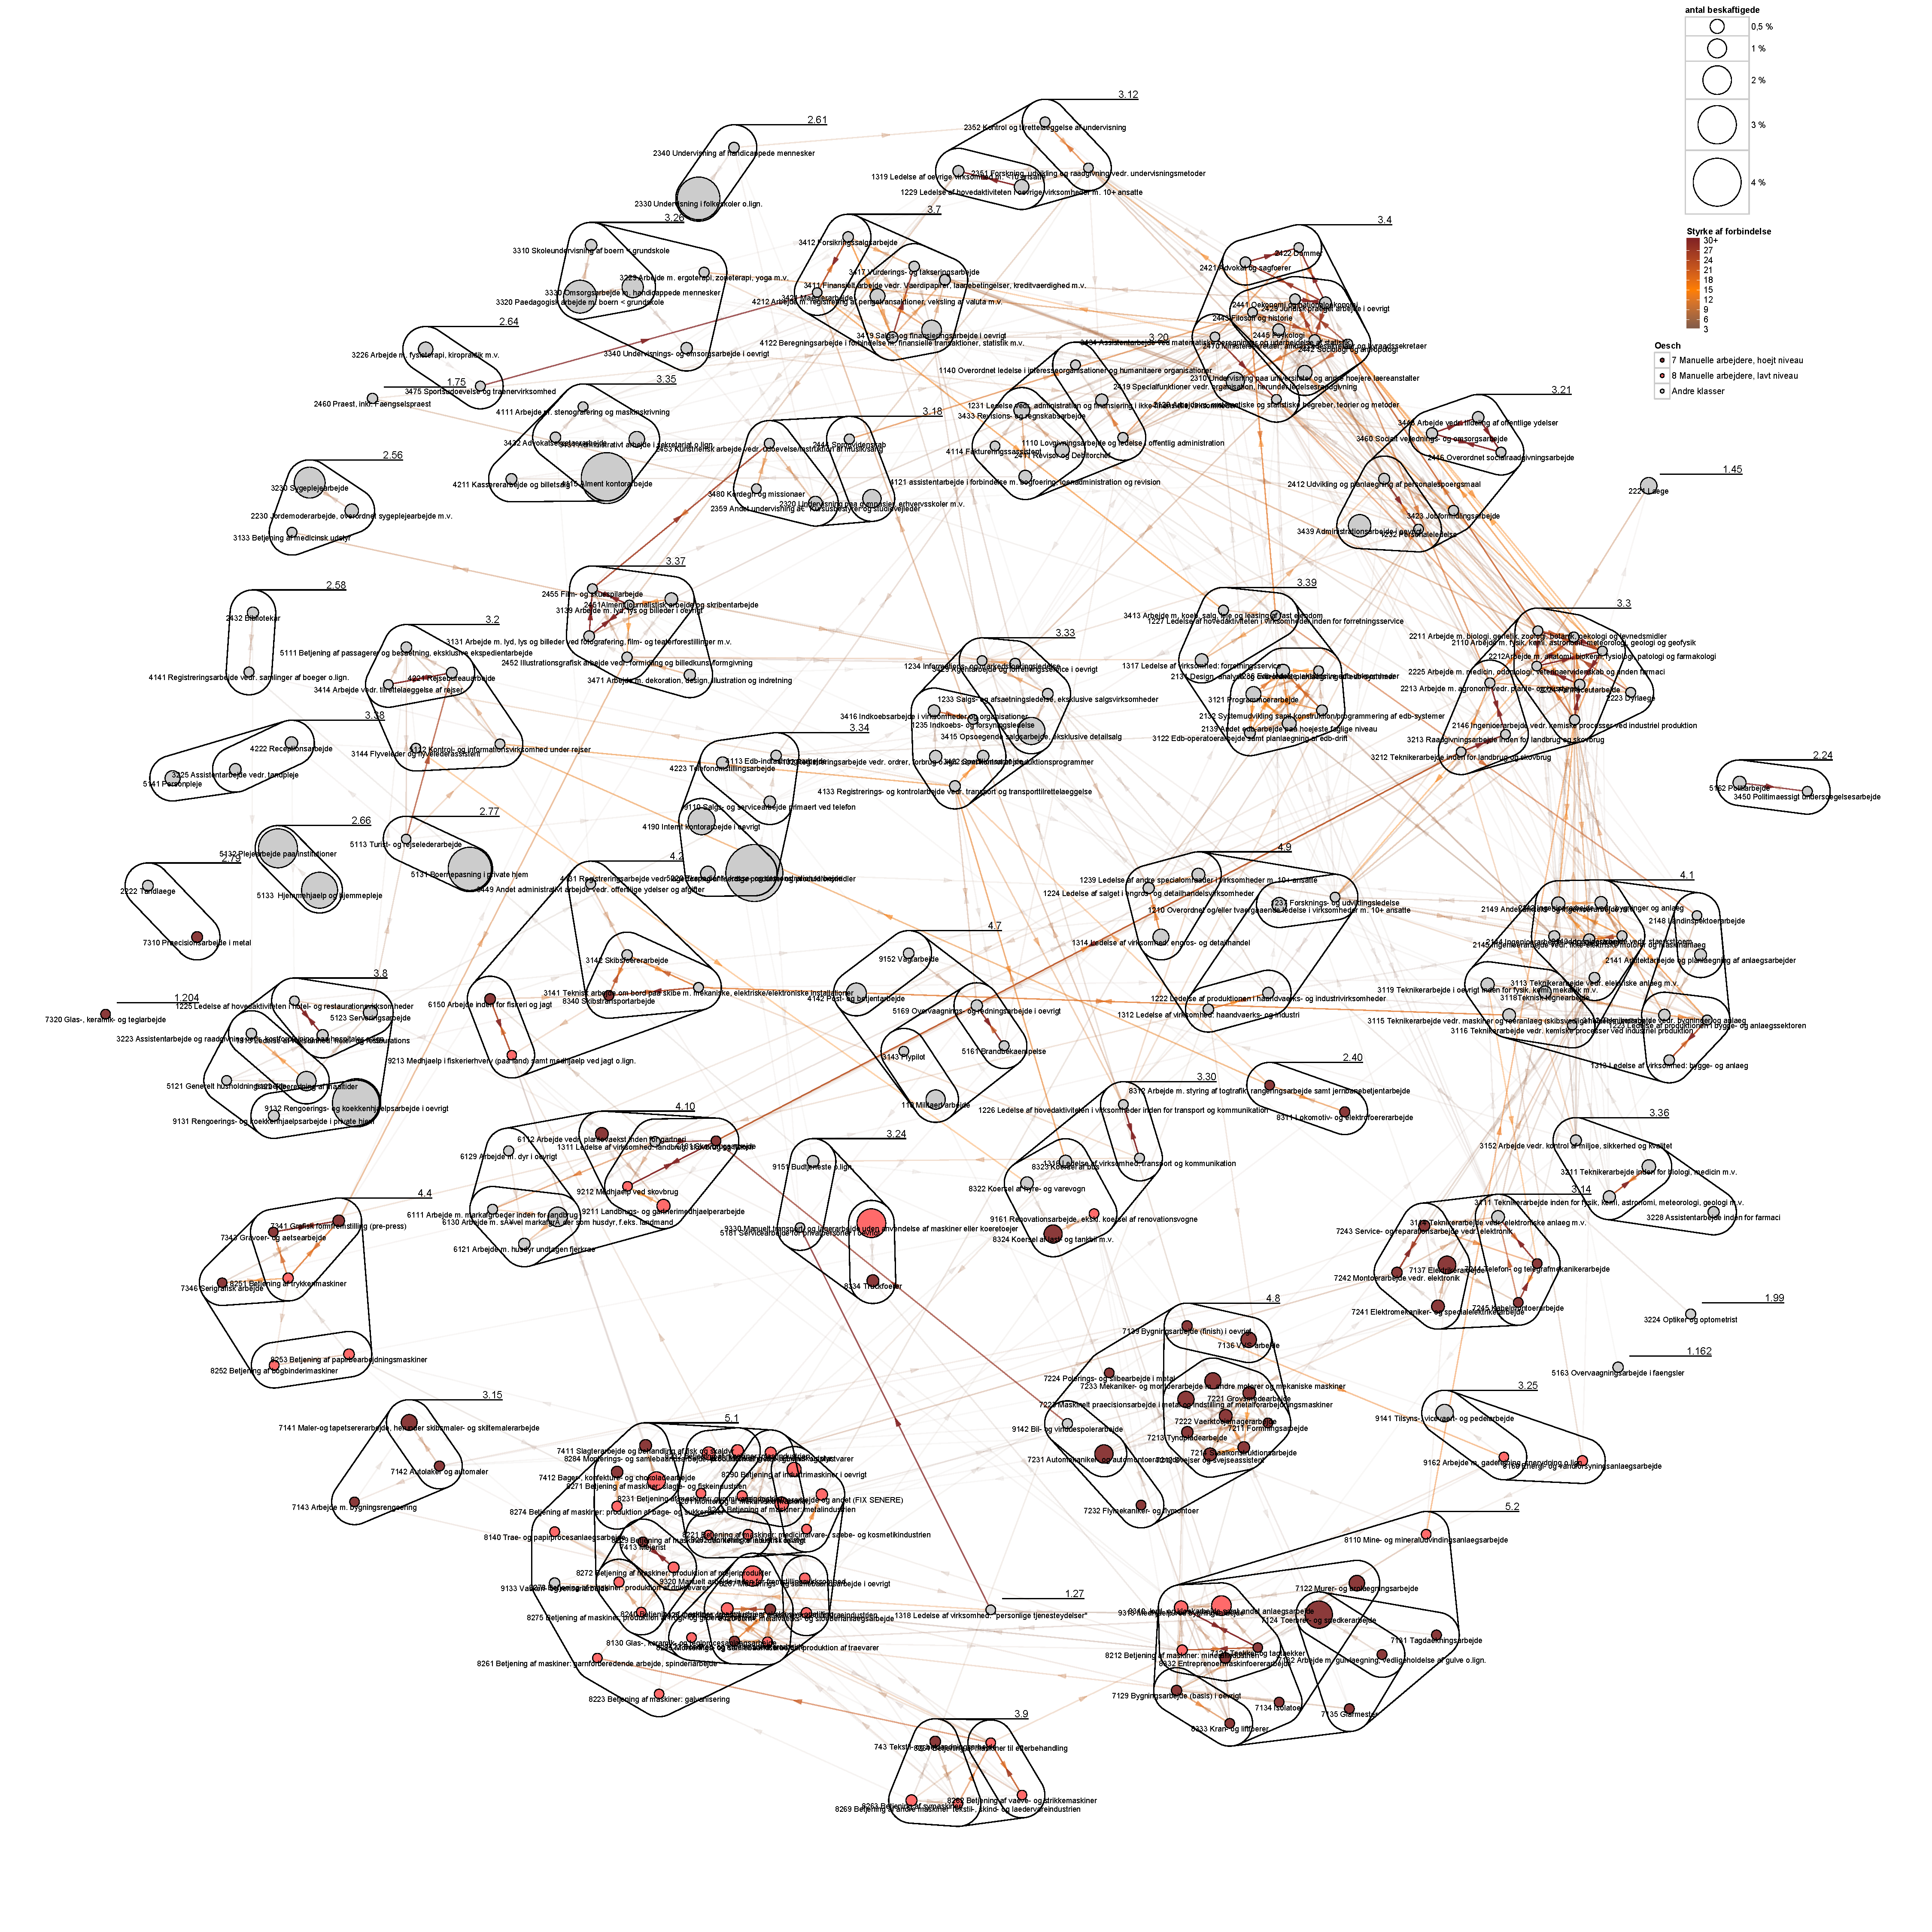
\includegraphics[width=\textwidth]{fig/netvaerkskort/kort_fokus_manuel_nonmanuel_roedgraa.pdf}
    \label{fig delanalyse3 klasse manuelt ikkemanuel}
   \end{centering}
   \end{figure}   
%


Langt de fleste af de erhvervsgrupper, der i Oeschs klasseskema er kategoriseret som manuelle arbejdere, er i samme segmenter. det ses også, at klassefraktionerne \emph{højere} og \emph{lavere} manuelt arbejde formår at at indfange de permabilitetsbarrierer, jeg tidligere har argumenteret for som centrale aspekter af hvad klasse er. Det er denne afhandlings unikke kombination af data på populationsniveau og en nyskabende netværksorienteret tilgang, der gør det muligt at undersøge dette aspekt af klasse. Det er derfor ganske spændende - og betryggende! at Oesch' klasseskema rent faktisk formår at ramme rimelig fornuftigt.

Der er imidlertidig undtagelser, der kan deles op i tre tendenser.

\underline{Den første tendens} omhandler de to, ganske vist manuelle, men højtspecialiserede erhvervsgrupper \emak{d7320} og \emak{d7310}. Disse to har en høj intern mobilitet på over 80 \%, og lader til at indfange en mesterlære-tradition, der fungerer effekt som social lukningsmekanisme. 

Dette er ikke specifikt for den manuelle arbejderklasse. Det er en trend, der ses indenfor de fleste klasser, eller, mere teknicistisk, hovedgrupper i Disco: Enkelte erhvervsgrupper formår at fungerere som selvstændige delmarkeder. Dette er ikke et centralt tema, men der er tydeligvis tale om en central del af arbejdsmarkedets struktur. Frank Parkin beskriver denne strategi som en strategi for at hæve egen markedsværdi, at erhvervet så at sige sørger for at have kontrol over egen arbejdskraft, og derved sikrer sig bedre vilkår og muligvis højere status end andre erhverv: “\emph{Professionalization itself may be understood as a strategy designed, amonst other things, to limit and control the supply of entrants to an occupation in order to safeguard or enhance its marked value}” \parencite[54]{Parkin1979}. Dette er ikke helt retvisende indenfor de to omtalte erhverv i den manuelle arbejderklasse, hvilket Parkin også skelner imellen. Professionelisering, e.g. adgangsgivende eksamener o.lign., er forskelligt alt efter om det sker som \emph{udbyttende} lukning, som indenfor højt bolige erhvervsgrupper såsom læger, eller om det er fagforeningsstrategier, hvis mål er at beskytte deres medlemmer mod udbytning. Forskellen er at det bevidste mål, i fagforeninger af den type Parkin mener, ikke har ævret at reducere de materielle muligheder for andre i arbejdsstyrken \parencite[57]{Parkin1979}. 
      % → det her skal stå et andet sted, i diskussionen, fx. For meget teori-tungt lige her. Bare kort i stedet, så det her ind et andet sted. 

\underline{Den anden tendens} handler om arbejdets genstandsfelt: Det ser ud til, at \emph{arbejdets genstandsfelt} er en betydningsfuld mekanisme i grænsedragningen mellem segmenter. Segment \emak{s4.10} og segment \emak{s4.2} har blandet klassesammensætning. Her er det henholdsvis landbrug og skibsdrift, der er genstandsfeltet, og det er muligt herigennem at skifte klasse. Jeg bruger bevidst ikke \emph{sektor} til at beskrive det, da disse genstandsfelter i en række tilfælde ser ud til at være for smalle til at kalde for sektor. Men det er tydeligt, at en sektor-baseret tilgang også har en del at sige om mobiliteten på arbejdsmarkedet. Man kan sige, at de fleste af segmenterne dækker et helt genstandsfelt, eller flere, \emph{i sig selv}: Og en håndfuld steder - der hvor et bestemt genstandsfelt dækker en relativt beskeden andel af alle beskæftigede, er en stringent seriel opdeling af arbejdsprocesserne ikke mulig. Det her, vi ser blandede klasse-segmenter, og hvor vi på segment-niveau kan se social mobilitet på tværs af de arbejdsfærdigheder, der et centralt aspekt af klassebegrebet (og disco-begrebet, og uddannelsesbegrebet etc). 

\underline{Den tredje tendens} er egentligt udtrykt for det samme som tendens nummer to. Forskellen er, at her indgår denne dynamik i den omstrukturering af beskæftigelsesstrukturen, som jeg beskrev i afsnit \ref{henvisning til Oesch}.  De manuelle erhvervsgrupper, der her er i segment med andre klasser, er den manuelle klasses \emph{transporterhverv}, og findes i \emak{s3.24} og \emak{s3.30}, sammen med de ligeledes transport-relaterede erhvervsgrupper fra Oesch serviceklasse. For at fortælle denne historie, skal vi se på ændringen i antallet af beskæftigede indenfor segmenterne over tid i perioden. 

Alt i alt findes der 3 segmenter, der primært eller udelukkende består af lavt manuelt arbejde, 5 segmenter og én erhvervsgruppe, der primært eller udelukkende består af højt manuelt arbejde, samt 5 segmenter, hvori de manuelle jobs er blandet med andre klassekategorier, hovedsageligt fra serviceklassen. 

En inddeling af den manuelle arbejderklasses segmenter i større fraktioner, baseret på de mobilitetsmønstre, som observeres, ser sådan ud: 

    %!TEX root = ../report.tex
%
\begin{table}[H] \centering
\caption[Manuel klasse: Fordeling af beskæftigede i segmenter]{Fordeling af beskæftigede for den manuelle klasses segmenter}
\label{tab delanalyse3 fordeling manuel}
\resizebox{0.8\textwidth}{!}{%
% Table generated by Excel2LaTeX from sheet 'tab_manuelklasse_seg_miks'
% Table generated by Excel2LaTeX from sheet 'tab_manuelklasse_seg_miks'
\begin{tabular}{lrrrrrr}
Klasse & Andel beskæftigede & Kummulativ andel & Antal segmenter & Andel segmenter & Antal erhvervsgrupper & Andel erhvervsgrupper \\
\midrule
Manuelle arbejdere, højt niveau & 13\%  & 13\%  &                 6  & 13\%  &               41  & 15\% \\
Manuelle arbejdere, lavt niveau & 8\%   & 20\%  &                 3  & 6\%   &               39  & 14\% \\
Manuelle arbejdere, højt/lavt miks & 1\%   & 21\%  &                 1  & 2\%   &                 6  & 2\% \\
\midrule
Manuelle arbejdere og andre klasser & 8\%   & 28\%  &                 5  & 11\%  &               27  & 10\% \\
Andre klasser & 72\%  & 100\% &               32  & 68\%  &            160  & 59\% \\
\midrule
I alt & 100\% &       &               47  & 100\% &            273  & 100\% \\
\end{tabular} }
\end{table}
% 

 
Her ser vi hvorledes den manuelle del af arbejderklassen er delt op, hvis vores udgangspunkt er dens segmentering i delmarkeder. Om de dele af arbejderklassen, der befinder sig i andre segmenter, bør inddrages, er et åbent spørgsmål. Mere om det senere, i første omgang vælger jeg at definere den manuelle klasse som bestående udelukkende af de segmenter, der kun består af klassens medlemmer. Dette mener jeg er formålstjenestligt, da de miksede segmenter, som jeg har været inde på, kan ses som:


%
\begin{enumerate}
 \itemsep -0.5em
   \item ikke tilhørende den manuelle klasse, dvs. forkert klassificeret i Oeschs skema
   \item Erhvervsgrupper, der befinder sig i klassens grænseområde%
   %
       \footnote{ Som Bourdieu siger i \emph{Refleksiv sociologi: (find citat, det med klasser er som der hvor flammen stopper ved ilden \#todo )}}%
   %
   \item Tilhørende den manuelle klasse, men er indlejret i afgrænsede produktionsenheder, vis specialiserede genstandsfelt giver dem kompetencer, hvori integration med andre klasser er mulig  
\end{enumerate}
%

Det vil jeg foreløbigt lade ligge, og i stedet konstatere, at vi ser at den manuelle klasse, i min noget snævrere definition, i perioden 1996 til 2009 i gennemsnit fylde 21 \% af arbejdsmarkedet, altså en ganske stor andel. 

Som jeg viste i afsnit \ref{fig teori tid Oesch8}, er tendensen i Danmark såvel som i andre vigtige vesteuropæiske lande, at andel af manuelt beskæftigede svinder ind, mens servicearbejdet stiger. Dette var imidlertidig ud fra Oeschs a priori klasseskema, der for det første er designet til at dække alle moderne, vestlige lande, men som ikke tager udgangspunkt i mobiliteten på arbejdsmarkedet. Jeg vil mene, at et sådant udgangspunkt gør det muligt at se nærmere på hvilke trends, der er at spore i klasseudviklingen, og det er til dette tidsaspekt, vi nu retter vores opmærksomhed mod.


%
\subsubsection{En forfaldshistorie? \emph{- den manuelle klasses diminituering} (dumt ord find bedre \#todo)}
%
 

I kapitel \ref{kapitel_teori_klasse}, figur \ref{fig teori tid Oesch8} på side \pageref{fig teori tid Oesch8} påviste jeg, hvordan Danmark følger samme overordnede mønster i beskæftigelsesstrukturen som de andre vesteuropæiske lande, som Oesch undersøger: Den manuelle arbejderklasse skrumper, mens serviceklassen øges. Nu har jeg så påvist påvist, at Oesch klasseskema i meget høj, nærmest perfekt, grad lever op til denne afhandlings \emph{reason d'etre}, mobilitetsbarrierer på arbejdsmarkedet. Dermed er det trivielt at konstatere, at de segmenter, klassen består af, \emph{også} falder. Det er dog mindre trivielt, og i høj grad \emph{også} denne afhandlings reason d'etre, hvis jeg kan sige det uden at misbruge den vending, at de konkrete beskæftigelser, som klassen består af, ikke nødvendigvis følger samme trend. At se på segmenter som jeg gør her, kan netop, i modsætning til ren klasseteori, være med til at give konkret forståelse af de erhverv, folk rent faktisk lever deres liv i. På et policy-plan er det meget konkret anvendeligt, at forstå hvordan man kan håndtere de delmarkeder, hvori flaskehalsproblemer opstår. I figur \ref{fig delanalyse3 klasse tid manueltsegment} ser vi udviklingen i den manuelle arbejderklasses segmenter over tid. 

%
   \begin{figure}[H]
   \begin{centering}
    \caption[Tidsserie: De manuelle arbejdersegmenter]{De manuelle arbejdersegmenter, udvikling i andel beskæftigede i perioden 1994-2009. Segmenter med < 1,5 \% beskæftigede er udeladt, af overskuelighedshensyn.} % du kunne lave en aggregeret gruppe med dem, og tegne dem som samlet gruppe. bare en ide, \#todo
    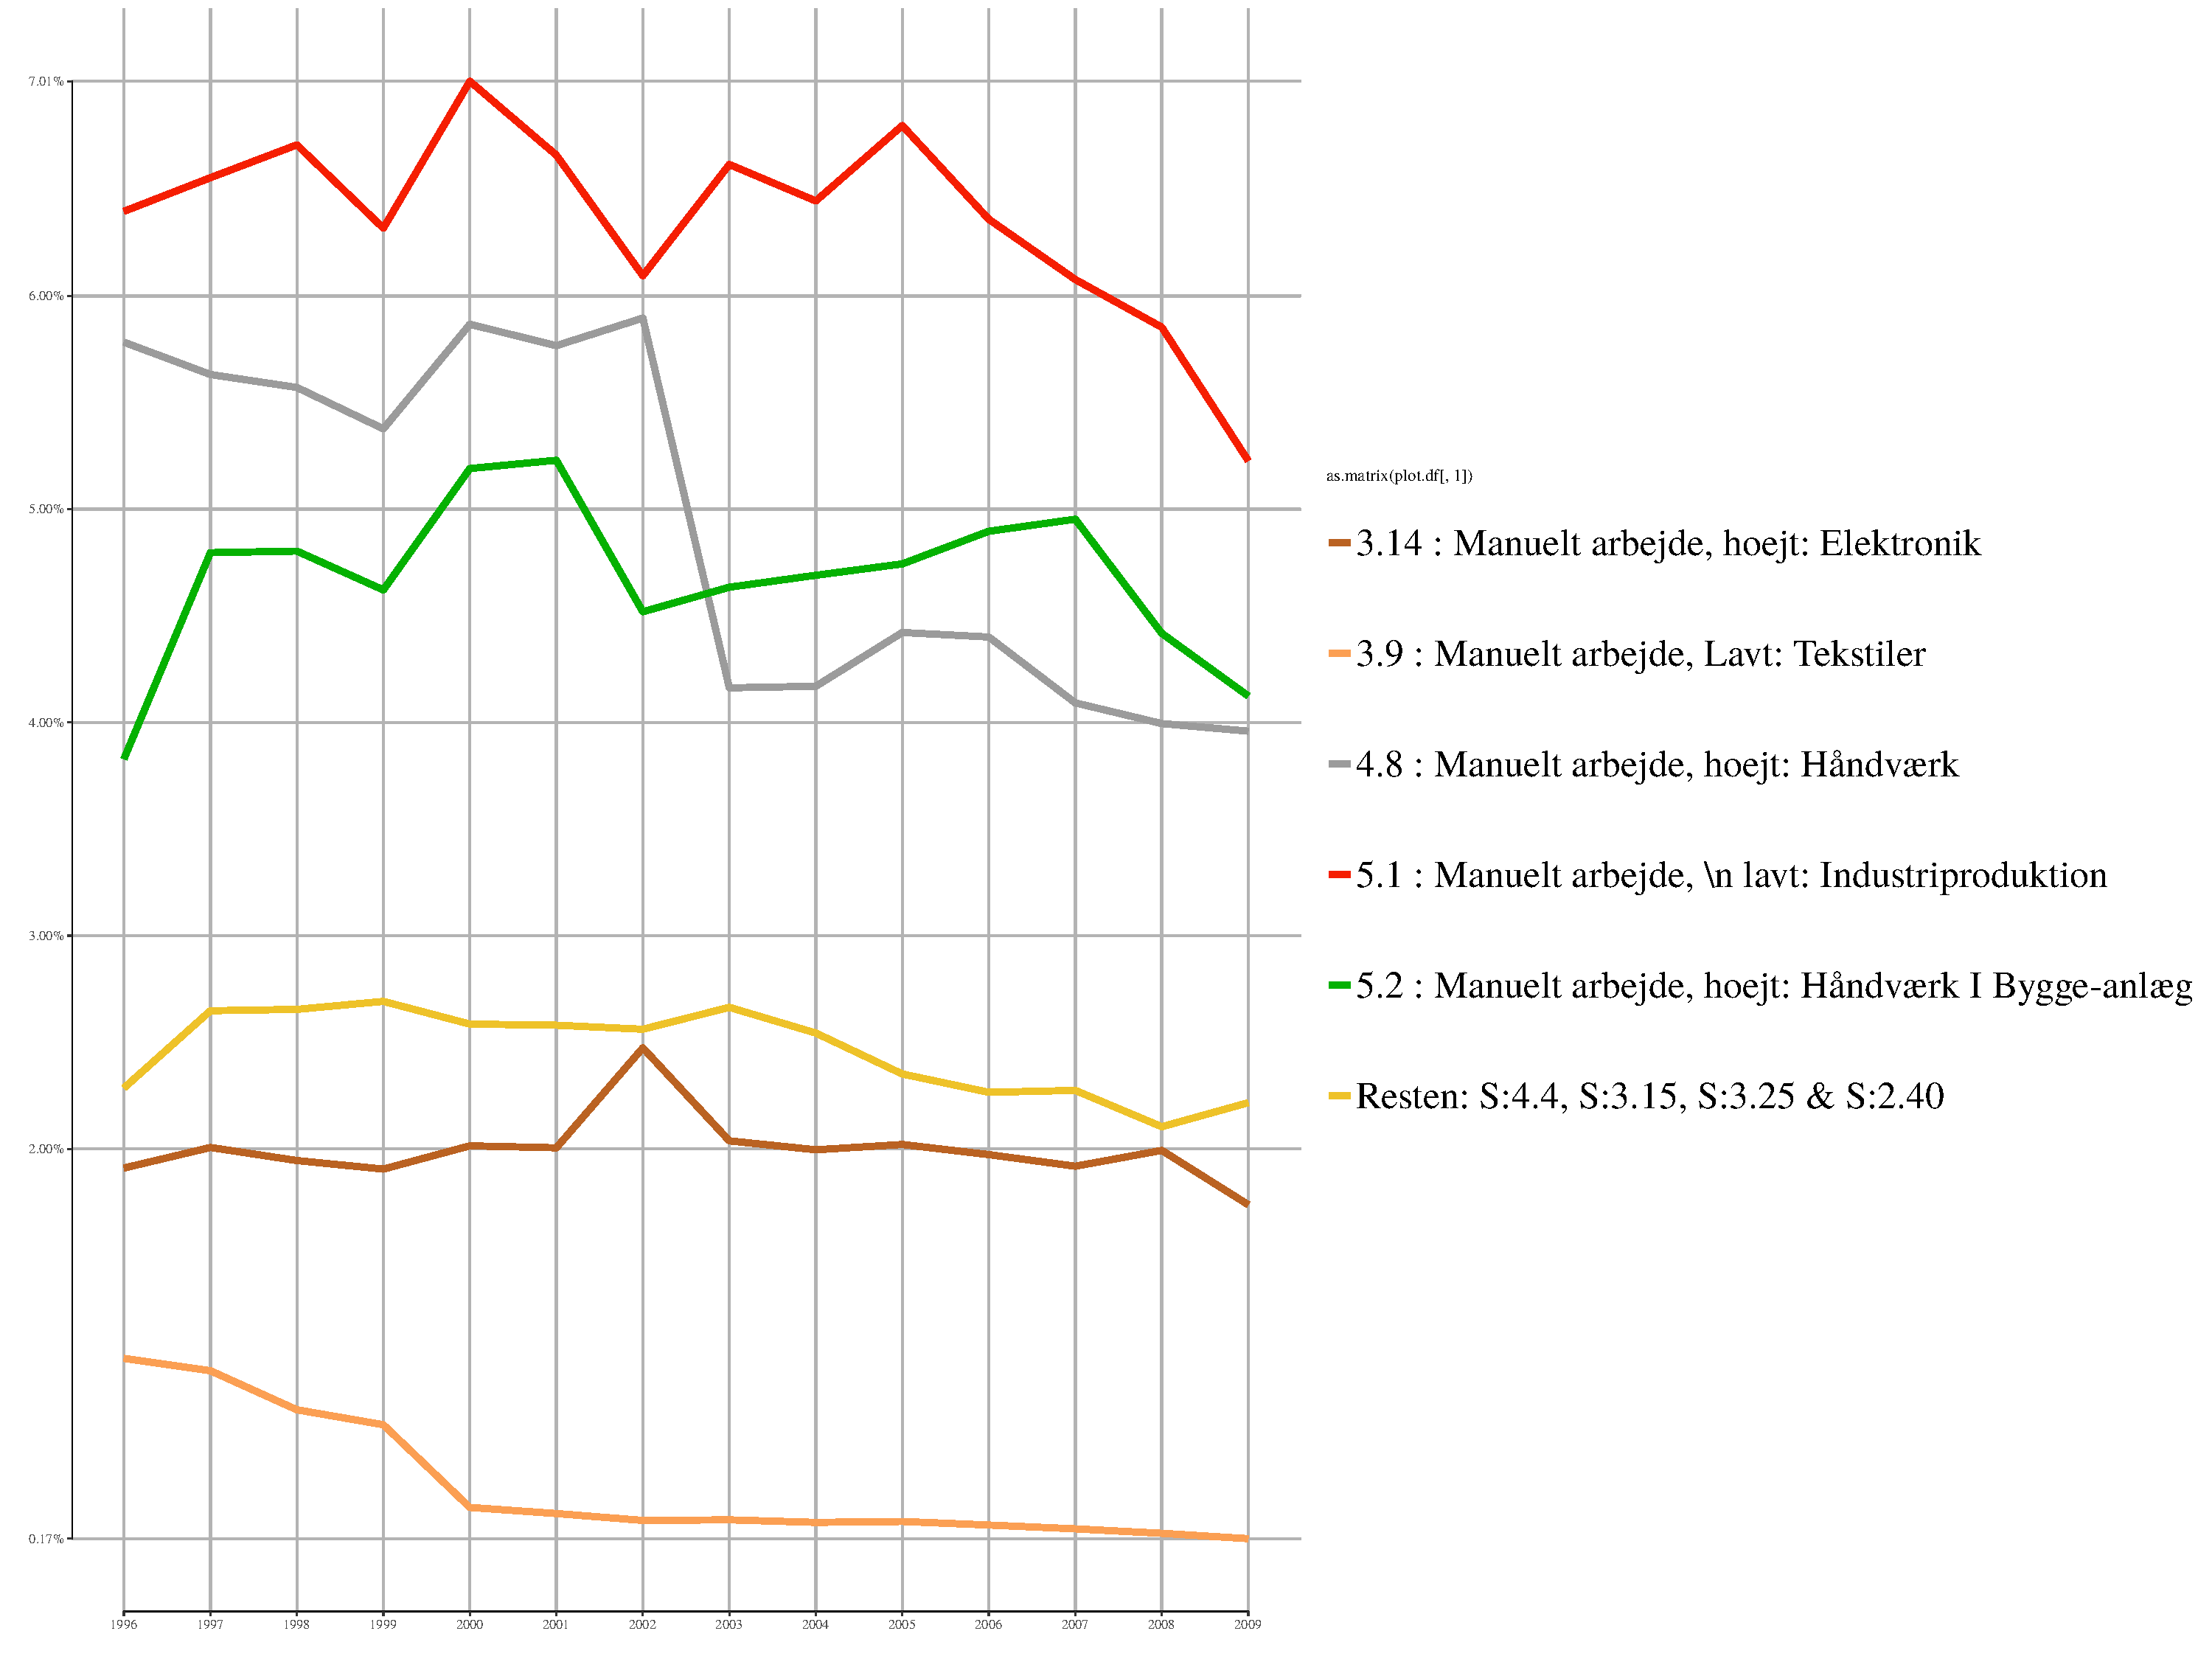
\includegraphics[width=\textwidth]{fig/tidsserier/tid_seg_manuelt.pdf}
    \label{fig delanalyse3 klasse tid manueltsegment}
   \end{centering}
   \end{figure}   
%

Vi lærer to ting ved at se på segmenterne. Det første er at det er 4 segmenter, der er drivkraften i tendensen til det støtte fald i manuelle jobs gennem midt-90'erne og 00'erne. To af ikke bare den manuelle klasses største segmenter, men \emph{hele arbejdsmarkedets}største segmenter, \emak{s5.1} og \emak{s4.8}, står for hele faldet%
%
    \footnote{ De to små segmenter \emak{s3.9} og \emak{s4.4} falder også i perioden, men er altså ikke afbilledet i figur \ref{fig delanalyse3 klasse tid manueltsegment} af hensyn til overskueligheden.}%
%
. Samtidig oplever \emak{s3.24} og \emak{s3.30} stigninger. Segment \emak{s3.24} er den ene af de to transport-klynger med manuelle arbejdere, og her er genstandsfeltet transport \emph{ af varer}. \emak{s3.30} oplever en mindre, omend stadig stabil, stigning i beskæftigelsen, og har at gøre med kørsel, der i mindre grad er fokuseret på varetransport. I denne klynge er det interessant, at ledelses-klasserne indenfor genstandsfeltet bevæger sig i samme \emph{segmentet} som de klasser, hvis arbejde de leder og fordeler.  


Det er tydeligt, at det særligt det traditionelle fabriksarbejde i \emak{s5.1} og bygge-anlægsarbejde har været på tilbagetog i perioden. Samtidig er det manuelle arbejde, der står for den eneste markante stigning indenfor klassen, et segment, der består af \emph{varetransport} på forskellig vis. 

Man kan diskutere, om dette segment egentligt hører til i den manuelle arbejderklasse. Dette vil jeg gemme til senere, men foreløbigt konstatere, der er noget om snakken, når vi taler om et tilbagetog for den traditionelle arbejderklasse. Det er lige så interessant, at bygge-anlægsjobs også forsvinder i en periode kendetegnet ved voldsom vækst og næsten fuld beskæftigelse (find tal \#todo). Her kan østudvidelsen af EU, og brugen af østeuropæisk arbejdskraft i sektoren, være en forklaringsfaktor. Dette speciale kan ikke afklare dette spørgsmål, men det er tydeligt, at selvom østeuropæisk arbejdskraft måske-måske ikke er en vigtig faktor i faldet i antallet af jobs i segmentet, så har erhvervsgrupperne i segmentet haft grund til at være bekymrede for deres jobposition. Jeg ser dette som et eksempel på, at en bestemt klasseposition giver visse erfaringer, der kan have en politisk effekt: Uanset om det er østeuropæisk arbejdskraft, muliggjort gennem EU, der er vigtigt her, så er den kobling lavet, og her bliver erfaringer fra arbejdslivet eventuel politiserende faktor, der kan forklare de lavtuddannedes EU-skepsis, og mulige stærkt indvandrerkritiske holdninger. På baggrund af de referede statikker og undersøgelser, mener jeg, at Moneca netop her viser at ved at se på mobilitetsklynger, som disse segmenter er udtryk for, ser vi, hvordan bestemte klassefraktioner har en fælles social oplevelse, indenfor deres type job, og dette gør dem, som vi kan se i undersøgelserne, mere tilbøjelige til at følge en bestemt klassehandlen, der ikke behøver være \emph{kollektiv refleksiv}. 

%
\subsection{Hvor går den manuelle klasse hen? \label{subsec delanalyse3 manuelle arbejdsklasse hvorhen mobilitet}}
%

Et af de spørgsmål, Denne metode er oplagt til at svare på, er hvilke mobilitetskanaler, der så findes mellem de forskellige segmenter. For at skabe bedre overblik over den sociale logik i disse mobilitetsmønstre, benytter jeg mig af et klassebaseret syn på arbejsmarkedets indretning. Jeg mener at et klassebaseret blik på arbejdsmarkedets forskellige positioner gør det nemmere at se, hvilke typer arbejde, der ligger socialt set nærmest for forskellige professioner, og det er mit formål at se, om jeg med dette blik er bedre i stand til at forklare disse mobilitetsmønstre.

Dette sigte har et dobbeltrettet formål: Man kan sige, at den empiriske ramme, med dets unikke fokus på mobilitet forstået ud fra netværksmetode, skal lære os at forstå noget om hvad klasse \emph{er} i dagens Danmark. Og Oeschs moderne klasseteori er et udgangspunkt, der tillader os at begribe den komplekse struktur, som Moneca viser os. 

Mobiliteten, særligt indenfor segmenterne, skal også gerne fortælle os noget, hvorvidt de teoretiske klasser, vi arbejder med, afspejler en social virkelighed, hvor mobilitet er “let og typisk”, som Weber sagde det. Så vurderingen går altså begge veje - fra klasse som måde at forstå mobilitetsmønstre på, og mobilitetsmønstre som en måde at forstå klasse på. 

I tabel \ref{tab delanalyse3 without.mob manuel} ses de segmenter, som den største andel af mobiliteten fra de manuelle segmenter går til.  Totalen på 78.897 er det antal skift, der findes fra de manuelle segmenter til andre segmenter, det vil sige \underline{uden} skift mellem eller internt i de manuelle segmenter. Den største kategori på “andre segmenter” samler 27 segmenter, hvor mobiliten fra den manuelle klynger hver for sig er under 5 \%, de fleste langt mindre. 
I alt bevæger personer beskæftiget i den manuelle klasse sig sig altså til 35 segmenter når de bevæger sig ud af den manuelle klasse, hvoraf det største antal skift til et segment er på 10.407 skift, mens det mindste er på 6 skift%
%
    \footnote{ ikke med i tabellen, men der er tale om den ikke-segmenterede, universitetsuddannelse \emak{d2221}.}%
%
. 

%
%!TEX root = ../report.tex

%
\begin{table}[H] \centering
\caption[Manuel klasse: Udadgående mobilitet]{Udadgående mobilitet for den manuelle klasse, målt i antal og andel skift}
\label{tab delanalyse3 without.mob manuel}
\resizebox{0.8\textwidth}{!}{%
\begin{tabular}{lrrrr}
      & \multicolumn{1}{c}{Udadgående mobilitet, } &       & \multicolumn{1}{c}{Kummulativ} & \multicolumn{1}{c}{Andel af total} \\
\multicolumn{1}{c}{Segment} & \multicolumn{1}{c}{antal skift} & \multicolumn{1}{c}{Andel} & \multicolumn{1}{c}{andel} & \multicolumn{1}{c}{antal skift} \\
\midrule
3.34: Service- og kontorarbejde. lavt &           10.407  & 13\%  & 13\%  & 1,1\% \\
4.7: Vagt- og sikkerhedsarbejde &             9.779  & 12\%  & 26\%  & 1,0\% \\
3.8: Restaurationsbranchen &             8.960  & 11\%  & 37\%  & 1,0\% \\
3.24: Varetransport &             8.678  & 11\%  & 48\%  & 0,9\% \\
4.1: Tekniker og ingeniørarbejde &             6.047  & 8\%   & 56\%  & 0,6\% \\
3.30 Vare- og persontransport &             5.348  & 7\%   & 62\%  & 0,6\% \\
2.77: Privat børnepasning og rejseleder &             4.688  & 6\%   & 68\%  & 0,5\% \\
2.66: Omsorgs- og plejearbejde &             3.863  & 5\%   & 73\%  & 0,4\% \\
Andre segmenter &           21.127  & 27\%  & 100\% & 2,2\% \\
\midrule
I alt &           78.897  & 100\% & 100\% & 8,5\% \\
\end{tabular}}
\end{table}
% 
%
% dit tal for absolut mobilitet er misvisende, fordi du ikke har sat mobilitet internt i segmenter til 0. Og det er jo det niveau, vi opererer på. Så gør det, eller fjern den kolonne. \#todo.

Mobiliten er særligt koncentreret om 4 segmenter: segment 3.34, 4.7, 3.8 og 3.24. Disse udgør 48 \% af den samlede mobilitet. Det er segmenter, hvoraf en stor del af erhvervsgrupperne er fra serviceklassens nedre del. Vi kan konstatere, at den påviste udvikling med væksten i servicearbejde









En betragtelig del af af mobiliten til \emak{s3.34} kommer fra   går fra \emak{s5.1}. 




%
\subsubsection{kort over den manuelle klasses bevægelser}
%

































skal vi zoome ind på de bevægelser, der går fra de manuelle arbejderes segmenter. figur \ref{fig delanalyse3 manuelklasse fokus} viser kortet over arbejdsmarkedet, hvor kun mobilitet \emph{fra} de manuelle klassesegmenter til andre segmenter er afbilledet%
%
    \footnote{ Det inkluderer bevægelser mellem de manuelle segmenter}%
%
. Læg mærke til at skalaen for forbindelsernes intensitet, målt i relativ risiko, er sat anderledes end i de tidligere kort, for at fremhæve også de “svagere” forbindelser%
%
    \footnote{ Husk på at en RR på 2,5, som er minimumsværdien på dette kort, stadig er over medianen på 2. Vi har stadig at gøre med \emph{særligt stærke} forbindelser.}%
%
. Erhvervsgruppernes farver er bestemt af klassesammensætningen af segmentet, de befinder sig i, sådan som jeg argumenterede for i det foregående afsnit. De manuelle klassesegmenter er mørkerøde. Den lave del af den manuelle klasse er lys rød, mens segmentet med et miks af de to fraktioner er mellemrød. De 4 segmenter hvori manuelle erhvervsgrupper indgår sammen med andre segmenter er orange. Alle andre klassesegmenter end de segmenter, der indeholder manuelle erhvervsgrupper, er grå. 

\begin{figure}[H]
\begin{centering}
  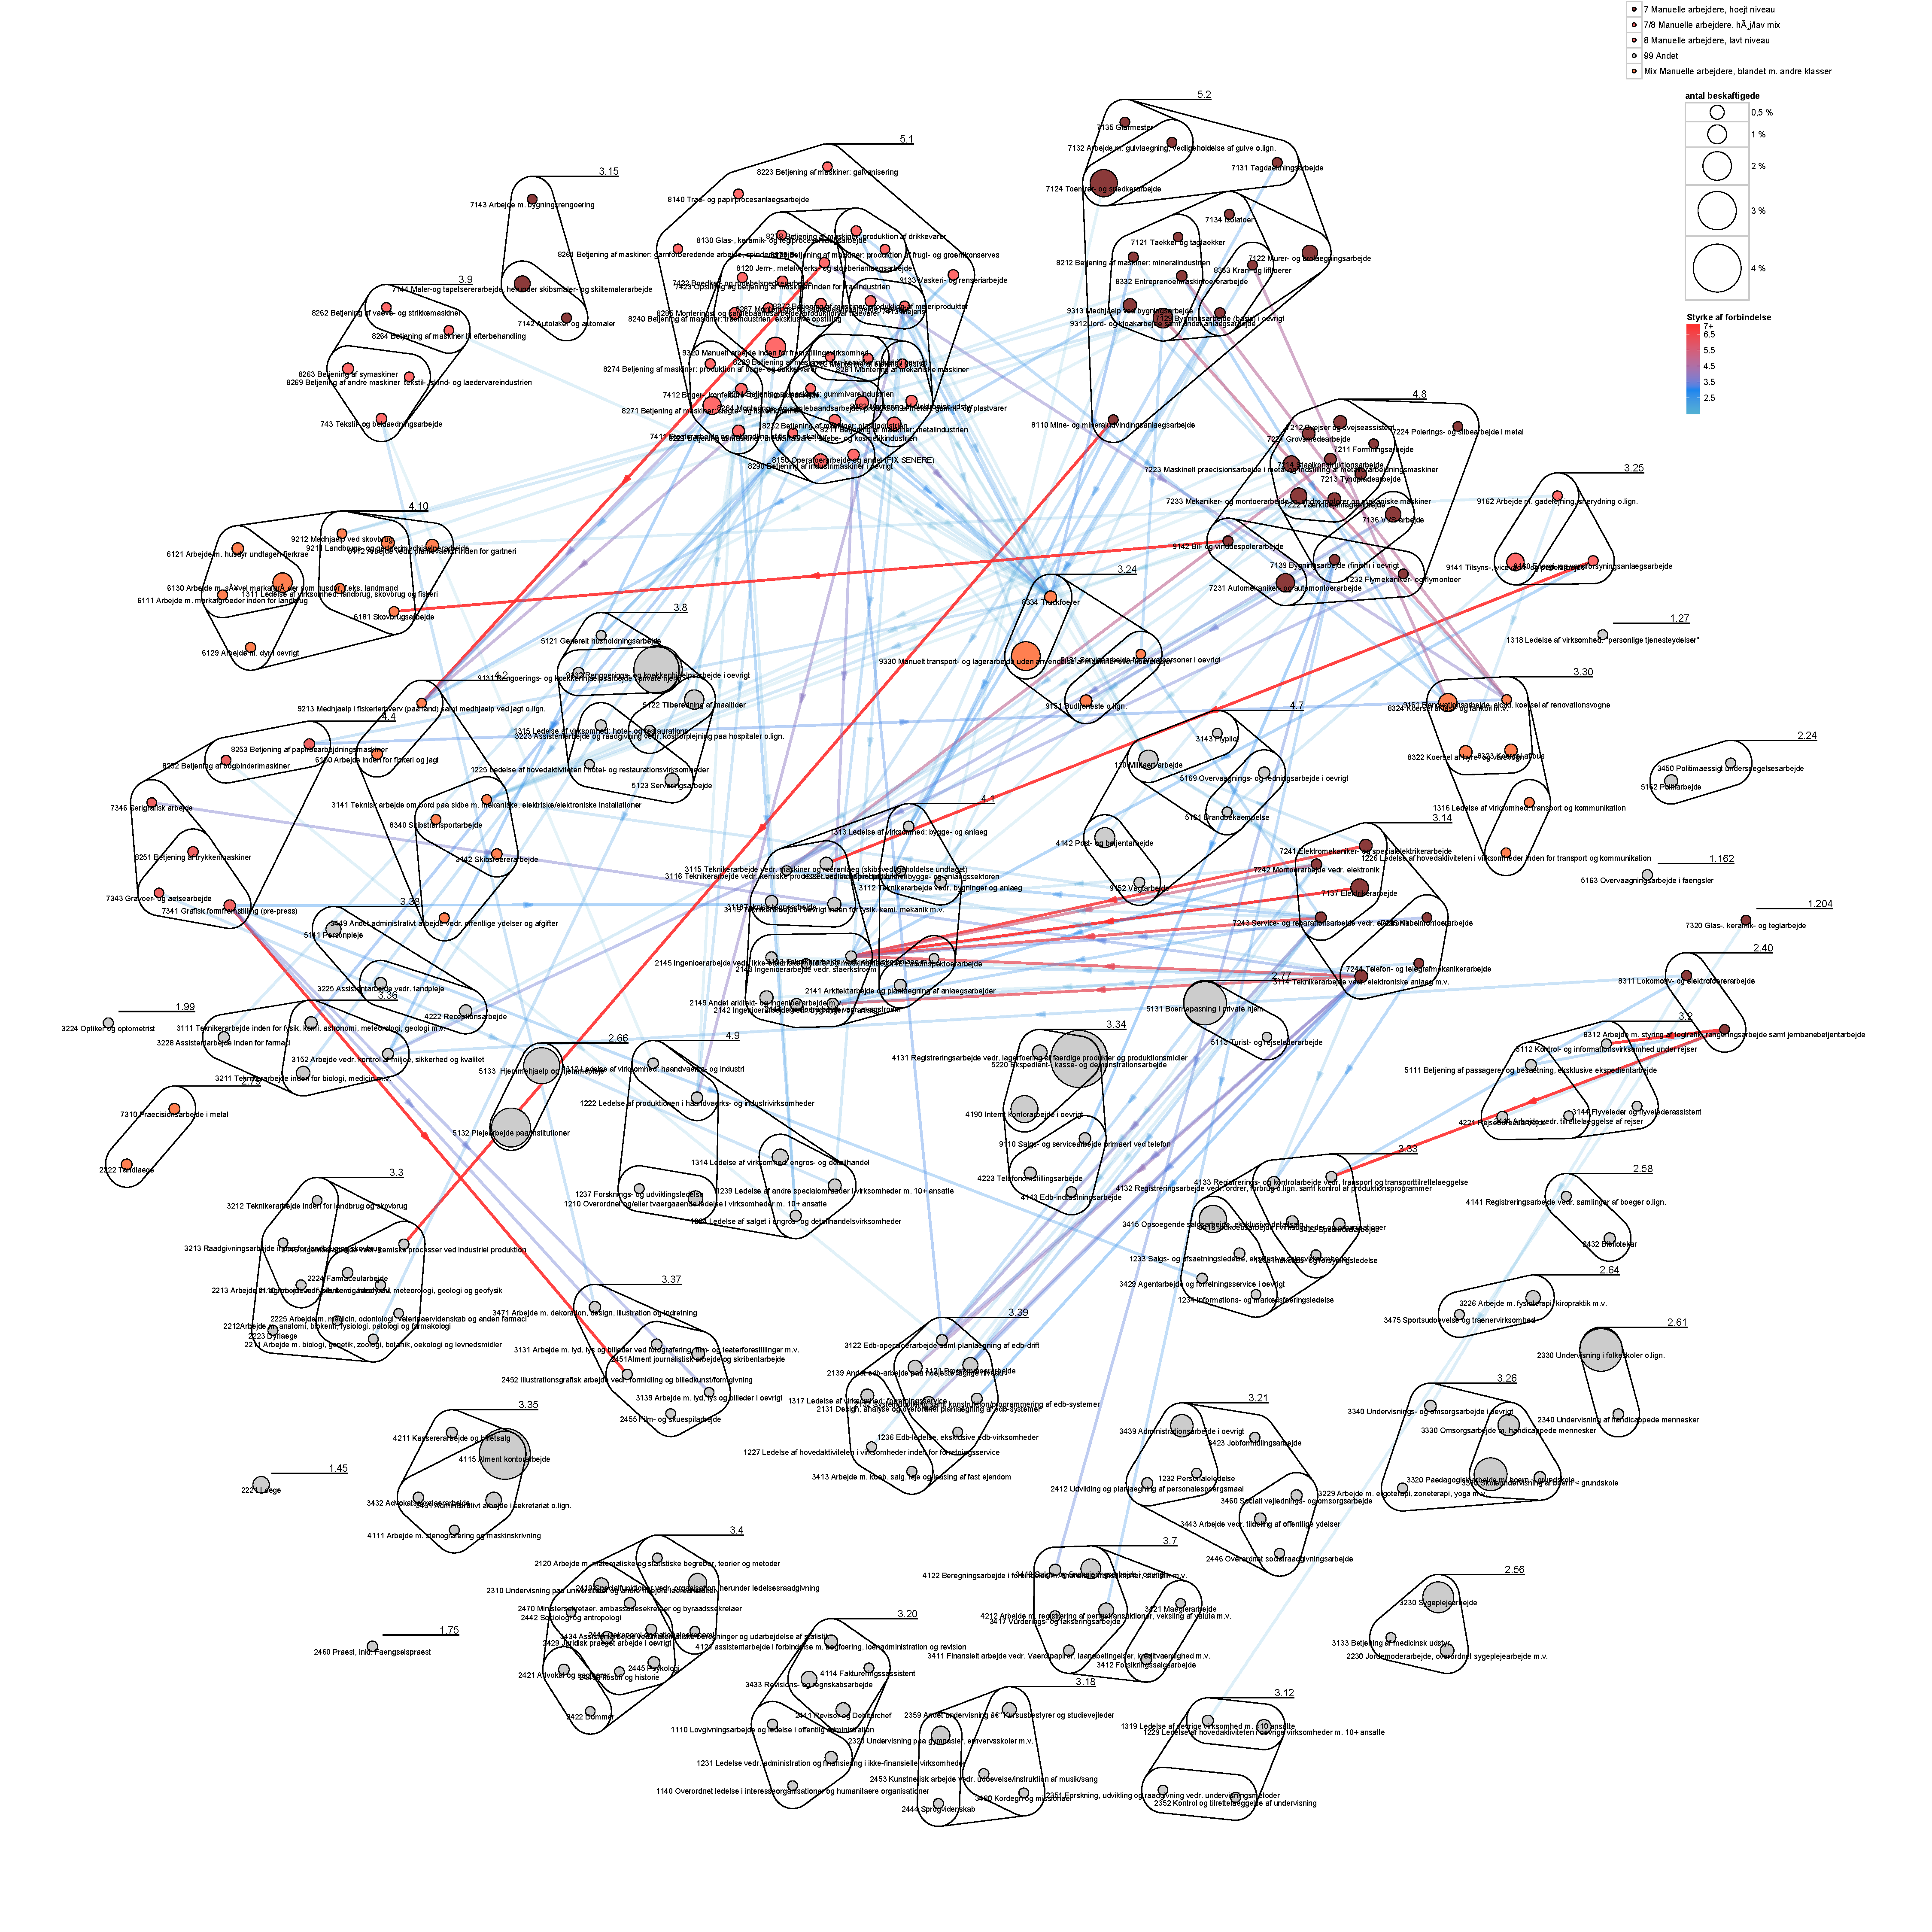
\includegraphics[width=10 cm]{fig/netvaerkskort/fokus_manuel_nonmanuel.pdf}
  \caption[Netværkskort: mobilitet fra den manuelle klasse]{Kort over de manuelle klasse-segmenters mobilitet til andre segmenter}
  \label{fig delanalyse3 manuelklasse fokus}
\end{centering}
\end{figure}

















%%%%%%%%%%%%%%%%%%%%%%%%%%%%%%%%%%%%%%%%%%%%%%
% #Noter 
%%%%%%%%%%%%%%%%%%%%%%%%%%%%%%%%%%%%%%%%%%%%%%
% 
% 
%
%

% En sidste overordnet betragtning om det kønnede arbejdsmarked, er at det ser ud til, at den kvindelige fabriksarbejder - altså kvinder beskæftiget indenfor manufaktur fremfor service - ser ud til at være forsvundet fra arbejdsmarkedet % brug kun denne reference hvis du kan finde en reference på hvor mange kvinder der arbejdede som fabriksarbejder i kapitalismens guldalder \#todo

% http://www.leksikon.org/art.php?n=1504
% og læs Marianne Rostgaards artikel om kvindelige og mandlige arbejdere op gennem det 20. århundrede.


policy-ide:
Man kunne: spore skiftene via registerdata, og lave sociale profiler på *hvem* der skifter *hvorhen*, så man bedst kan vurdere, om det er smart






\iffalse \label{iffalse}
%%%%%%%%%%%%%%%%%%%%%%%%%%%%%%%%%%%%%%%%%%%%%%%%%%%%%%%%%%%
% Trash 

%%%%%%%%%%%%%%%%%%%%%%%%%%%%%%%%%%%%%%%%%%%%%%%%%%%%%%%%%%%








\fi


